
\subsubsection{フロアマップを用いた歩行可能座標への補正}
% TODO: 3.座標よりも座標の方がいいかもしれない

図\ref{fig:pdr-rotate}に示す軌跡には、人間が歩行不可能なを通過している
という重要な問題が残されている。

図\ref{fig:unwalkable_points}は歩行可能な座標を青色の点,
歩行不可能な座標を赤色の点を可視化したものである.
\begin{figure}[H]
    \centering
    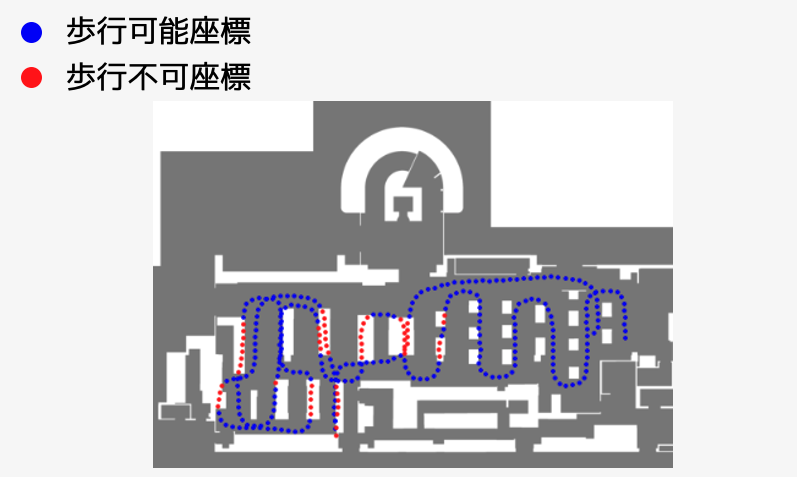
\includegraphics[width=\linewidth]{image/unwalkable_points.jpg}
    \caption{}    \label{fig:unwalkable_points}
\end{figure}


図\ref{fig:pdr-rotate}に示す軌跡には、人間が歩行可能座標ではない場所を
通過しているという重要な問題が残されている。図\ref{fig:walkable-points}は
ある軌跡上の点が歩行可能な座標であるか否かを示している。青色の点は
歩行可能な座標上に存在する点を、赤色の点は歩行可能ではない座標上に
存在する点を表している。この図から分かるように、軌跡の一部が壁や
障害物の存在する座標を通過している。このような軌跡は人間の実際の
歩行経路としては物理的に不適切である。この問題に対処するため、
本ライブラリではMapMatcherクラスの歩行可能座標補正機能を提供している。


この手法を利用するために必要な情報は、前節と同様のフロアマップ情報である。
このマップ情報を用いて、軌跡上の各点が歩行可能な座標に存在するように
補正を行う。

この手法の利用例を以下に示す:

\begin{lstlisting}
# MapMatcherの初期化
map_matcher = MapMatcher(
    pdr_estimator=estimator,  # PDREstimatorインスタンス
    floor_map=floor_map      # フロアマップ情報
)

# 歩行可能座標への補正
walkable_trajectory = map_matcher.correct_unwalkable_points(trajectory)
\end{lstlisting}

補正処理は以下の手順で行われる。まず、軌跡上の各点について、その座標が
フロアマップ上の歩行可能座標に存在するかを判定する。ある時刻$t$の
座標$(x_t, y_t)$が歩行不可能な座標に存在する場合、その点から最も近い

歩行可能な座標$(x_t^*, y_t^*)$を探索する。

この探索には幅優先探索(BFS)アルゴリズムを用いる。具体的には、現在の
座標から上下左右および斜め方向に探索を行い、最初に見つかった歩行可能な
座標を$(x_t^*, y_t^*)$として採用する。この際、探索はマップの境界を
超えないように制限される。

歩行可能な座標が見つかった場合、時刻$t$以降の全ての軌跡の座標を、
以下の式に従って平行移動する:

\begin{equation}
x_k' = x_k + (x_t^* - x_t), \quad y_k' = y_k + (y_t^* - y_t) \quad (k \geq t)
\end{equation}

ここで、$(x_k', y_k')$は補正後の座標、$(x_k, y_k)$は補正前の座標を表す。
この処理により、歩行不可能座標に存在していた点とそれ以降の軌跡が、
最も近い歩行可能な座標へと移動される。

この補正処理は軌跡の始点から順に適用される。図\ref{fig:map-matching}に
示すように、補正後の軌跡では全ての点が歩行可能な座標内に存在している。
なお、この補正処理は前節までの補正とは異なり、軌跡の進行方向は保持
したまま、位置のみを補正する特徴がある。

\begin{figure}[H]
    \centering
    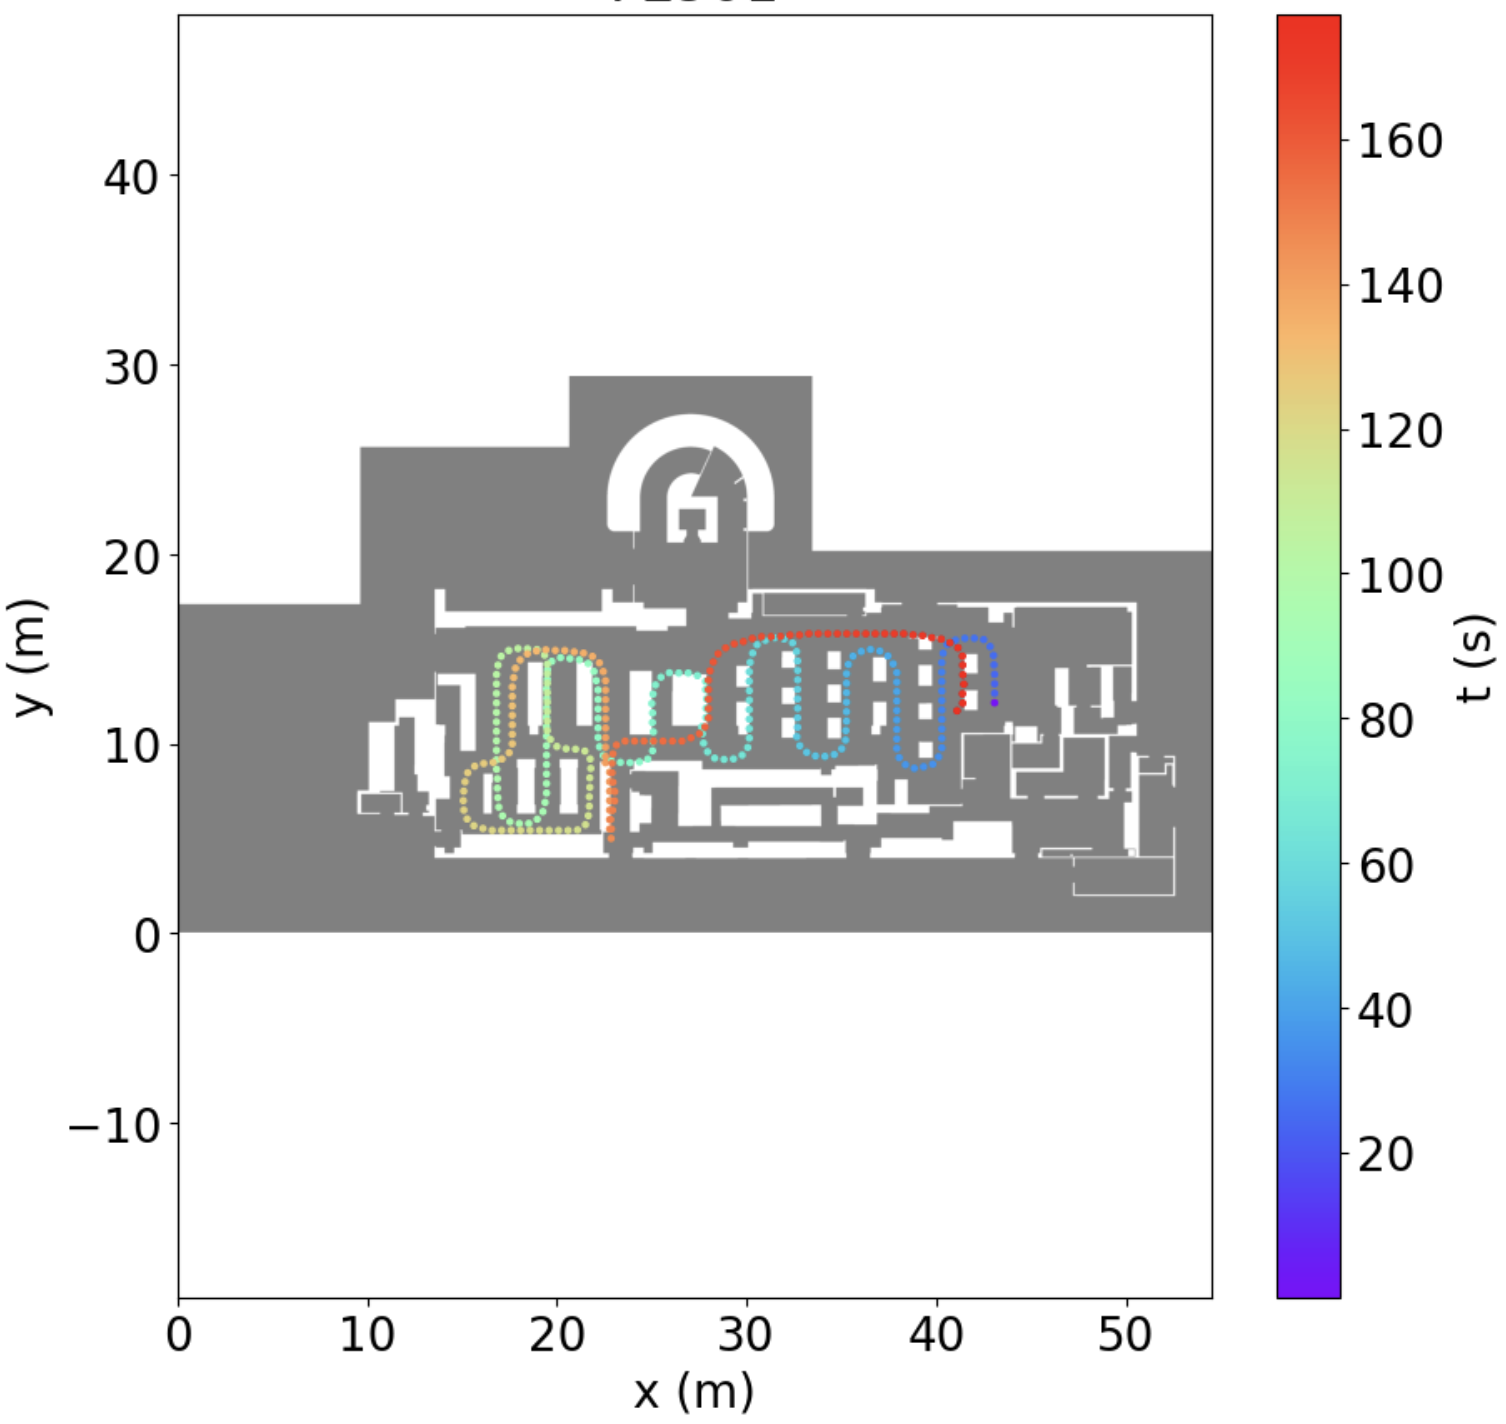
\includegraphics[width=\linewidth]{image/map-matching.jpg}
    \caption{マップマッチング補正後の軌跡}    \label{fig:map-matching}
\end{figure}
